\section{Experimentation}

% The best-produced model, the anchor-free YOLOv8-X model, achieved a mAP50 of 99.5\% and a mAP50-95 of 85.6\% on the test set with an inference time of 21.7ms, approximately 46 frames per second (FPS), demonstrating its effectiveness in real-time surgical tool detection. The proposed tracking algorithm has an accuracy of 100\% over the detected tools and too.tipsl These results highlight the potential of the models for accurate tool localization, even in resource-constrained environments.

\subsection{In-House Dataset}

% describe the flow of participants throughout the study

% number of participants

% outcome overall: Clear differences in some images (see differences in Test1 and Test2 scenes, and cut off images in Test2. Overheating in camera causing some image defects. edges more distinct, exact SOTA for opposite (YOLO in IRL, SIMO for ART)	 

% summary of follow-up

% overall characteristics of data source and setting

% we further used the best performin model to generate annotations for the rest of the dataset

\begin{figure}[htbp]
    \centering
    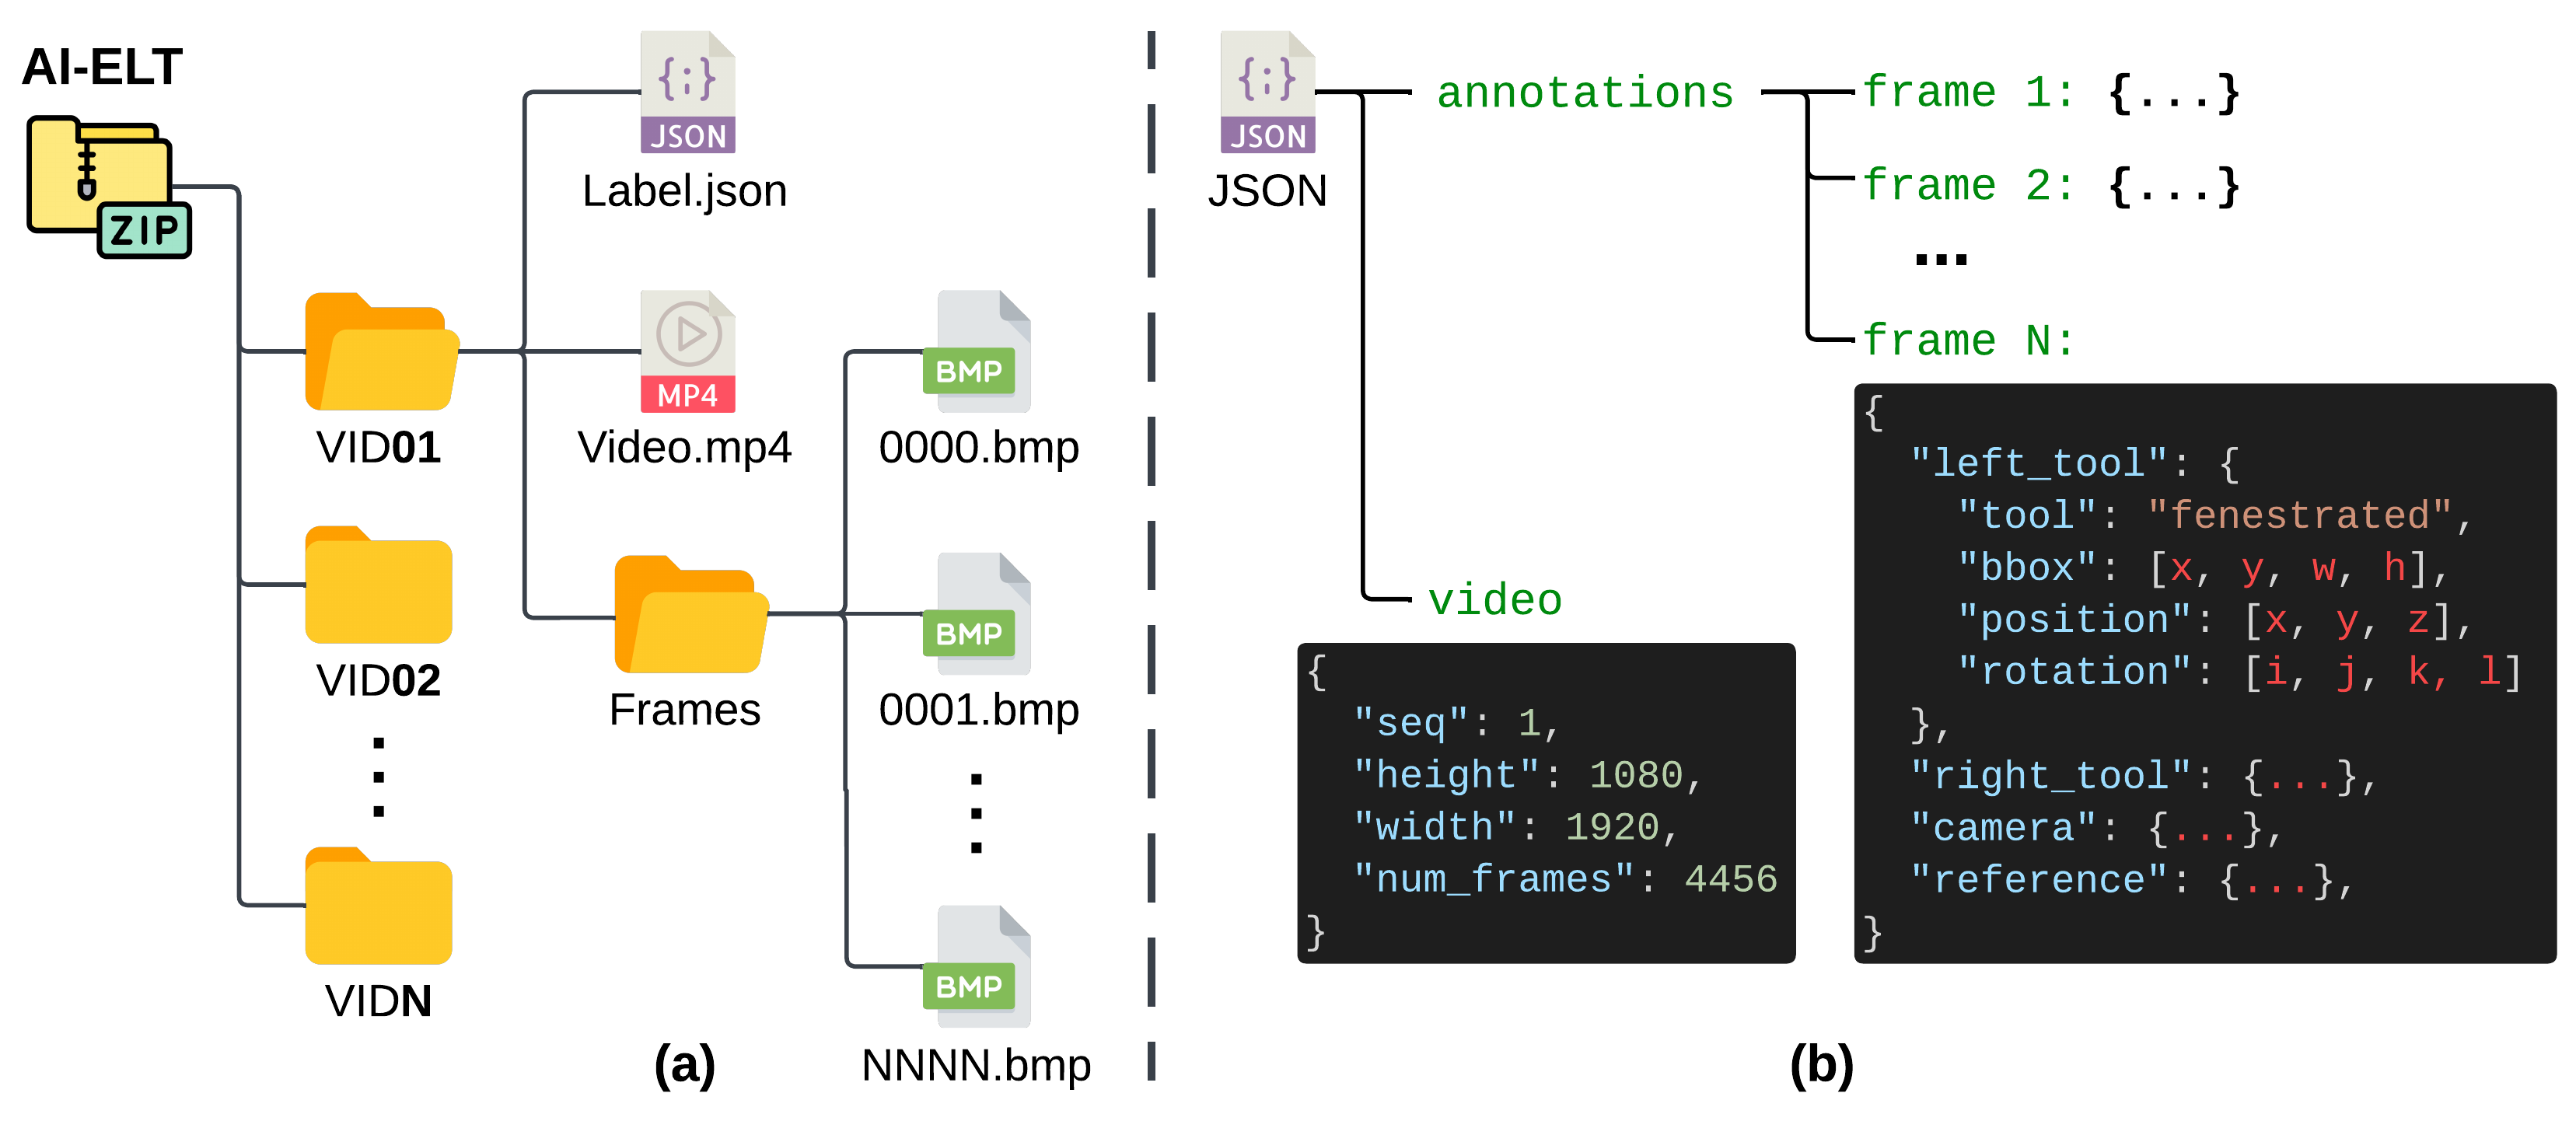
\includegraphics[width=\linewidth]{schematic_diagram.png}
    \caption{Schematic diagram of the dataset files showing (a) folder structure for the dataset and (b) Data structure for the JSON label files.}
    \label{fig:schematic_diagram}
\end{figure}

Inspired by the CholecTrack20 schematic diagram \cite{nwoye_cholectrack20_2023}, we present an intuitive way to understand the dataset.

The average number of procedures performed was 120, with a range of 0 to over a 1000, with 22 estimated to be performed on average in the last 12 months, ranging from 0 to 100. All 24 participants agreed to share their results entirely. If we categorise the surgeons skill based on number of procedures, were low is <20, medium is between 20 and 100 and high is >100, then we have 9 low, 9 medium and 6 high skilled surgeons. Results from the Edinburgh Handedness survey \cite{oldfield_assessment_1971} showed almost all surgeons were right-handed, with one left-handed (participant 12) and one who alternated hands (participant 3).

\subsubsection{Data Annotations}

% overall data annotated

% issues faced

\subsection{Model Configurations}

We have specifically designed the models with helper functions throughout the repository, freely available for assistance in future development.

\subsubsection{Anchor-based Model}

\subsubsection{Anchor-free Model}

\subsection{Training Setup}

\subsection{Model Evaluation}

% IoU, mAP50, mAP50-95, MSE

\subsection{Results}

% discuss differences between SIMO and YOLO models

\subsubsection{Surgical Tool Detection}

% IMAGE: bounding box tool and tooltips

% DIAGRAMS

\subsubsection{Surgical Tool Tracking}

% IMAGE: show tracking of tool (bounding boxes over time)

% DIAGRAMS

\subsubsection{Performance of the Model}

% YOLO10 architectures
% tested with all data - overfit too easily

% SIMO - initial issues, like segmentation, changed to detection with confidence values, added FCN

% main discoveries

\subsubsection{Comparison to Previous Work}

\subsubsection{Qualitative Results}

% Summary of what we saw in the results. main discoveries